%\pagebreak

\subsection{Evidencia de realizaci\'on}
Como evidencia se presentan las figuras 1 a 9, las cuales muestran la velocidad registrada por el
estroboscopio y el comportamiento de la se\~nal a dichas velocidades. Tambi\'en se anexa al final
del reporte la hoja de c\'alculos con los datos registrados.

  \begin{figure}[!htbp]
 \centering
 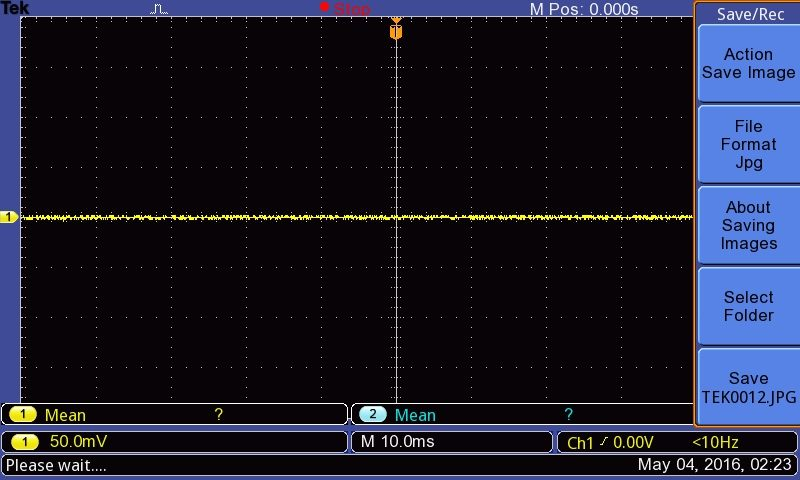
\includegraphics [scale=0.25]
 {./img/tek0012.jpg}
  \caption{Ruido detectado por el osciloscopio.}
 \end{figure}

 \begin{figure}[!htbp]
 \centering
 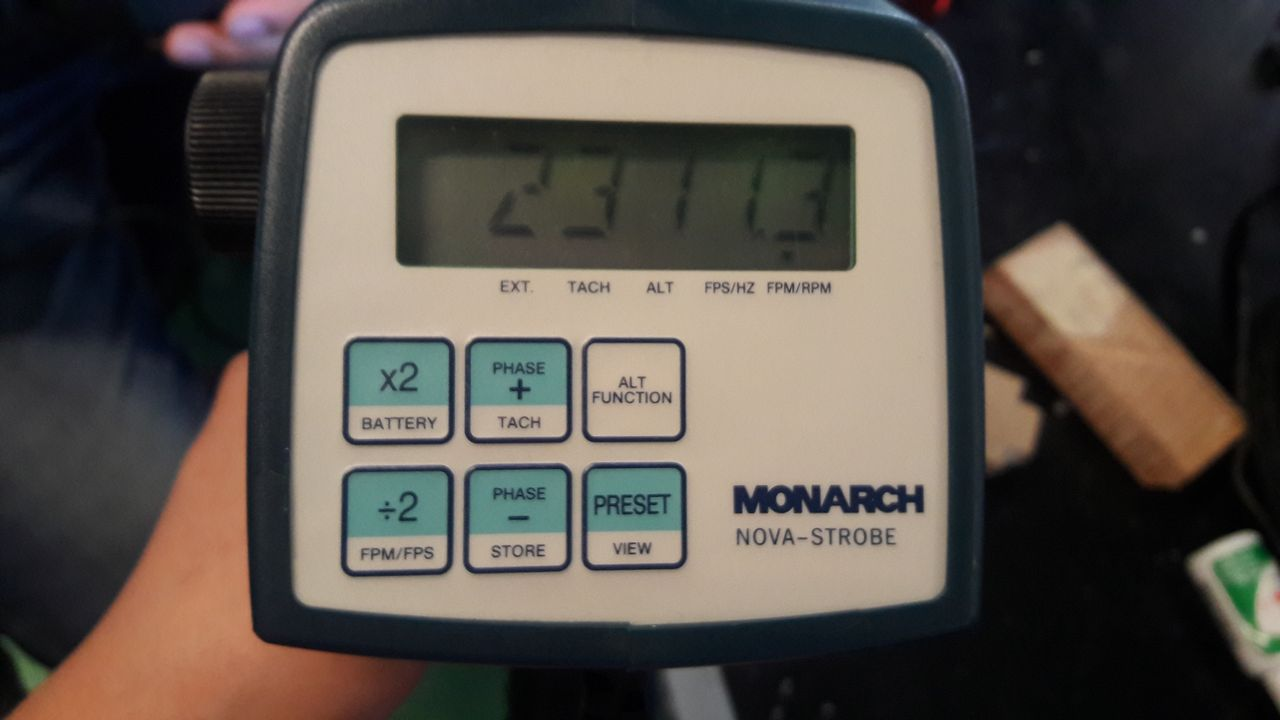
\includegraphics [scale=0.2]
 {./img/2311.jpg}
  \caption{Operaci\'on a 25\% de velocidad.}
 \end{figure}

  \begin{figure}[!htbp]
 \centering
 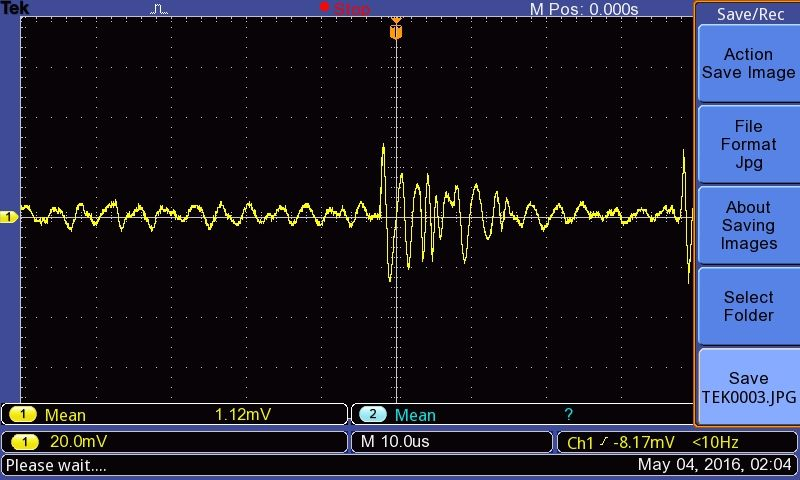
\includegraphics [scale=0.25]
 {./img/tek0003.jpg}
  \caption{Se\~nal a 25\% de velocidad.}
 \end{figure}

  \begin{figure}[!htbp]
 \centering
 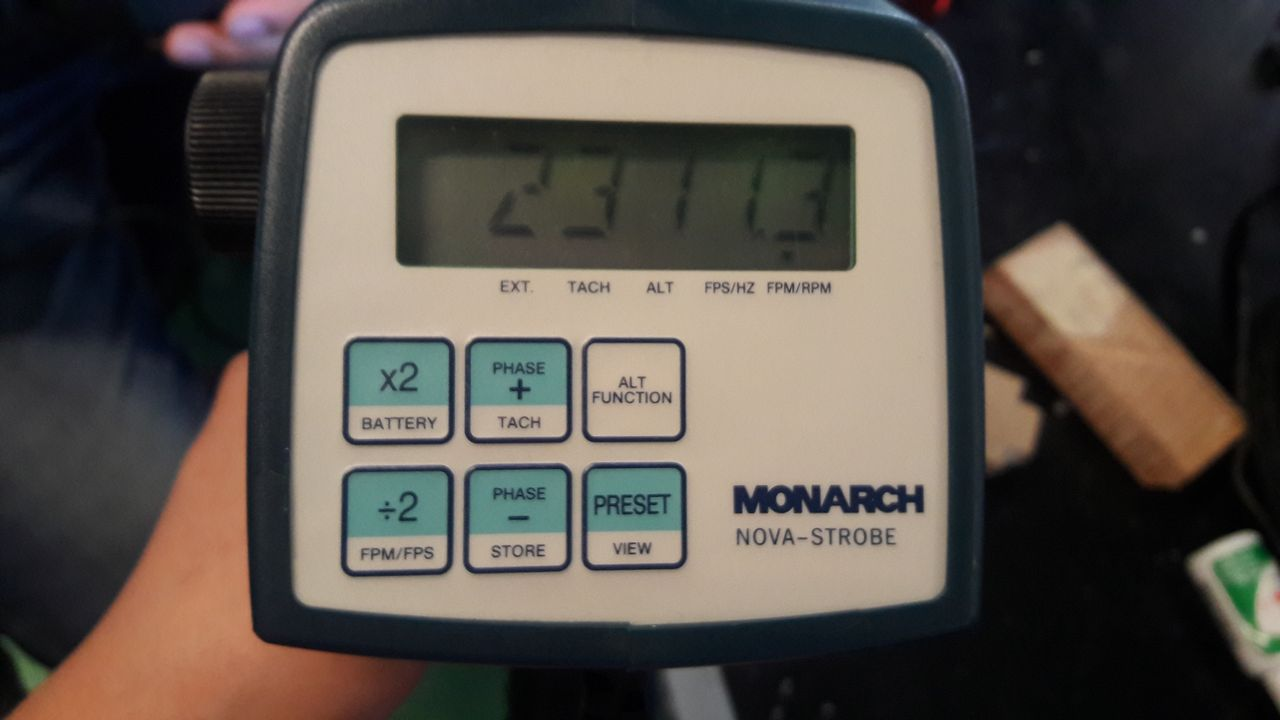
\includegraphics [scale=0.2]
 {./img/2311.jpg}
  \caption{Operaci\'on a 50\% de velocidad.}
 \end{figure}

  \begin{figure}[!htbp]
 \centering
 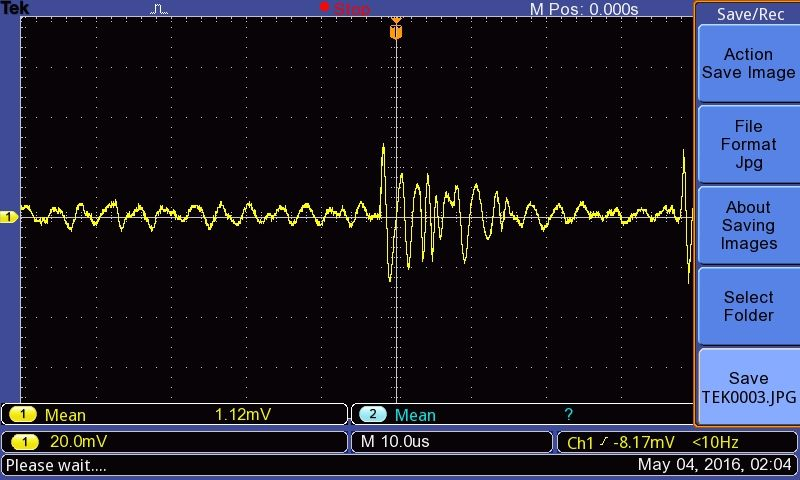
\includegraphics [scale=0.25]
 {./img/tek0003.jpg}
  \caption{Se\~nal a 50\% de velocidad.}
 \end{figure}

  \begin{figure}[!htbp]
 \centering
 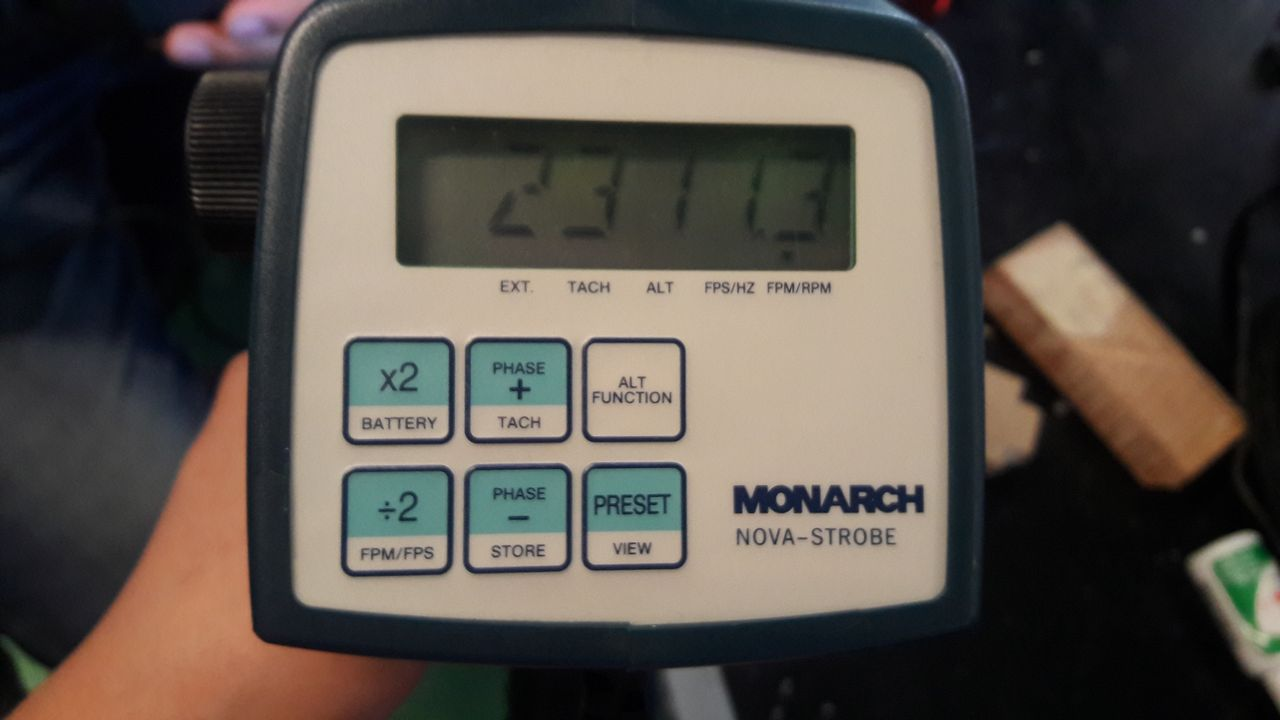
\includegraphics [scale=0.2]
 {./img/2311.jpg}
  \caption{Operaci\'on a 75\% de velocidad.}
 \end{figure}

  \begin{figure}[!htbp]
 \centering
 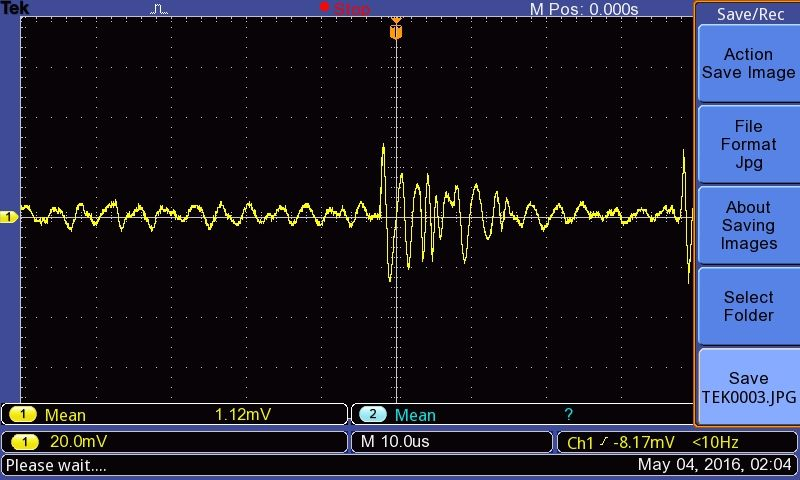
\includegraphics [scale=0.25]
 {./img/tek0003.jpg}
  \caption{Se\~nal a 75\% de velocidad.}
 \end{figure}

  \begin{figure}[!htbp]
 \centering
 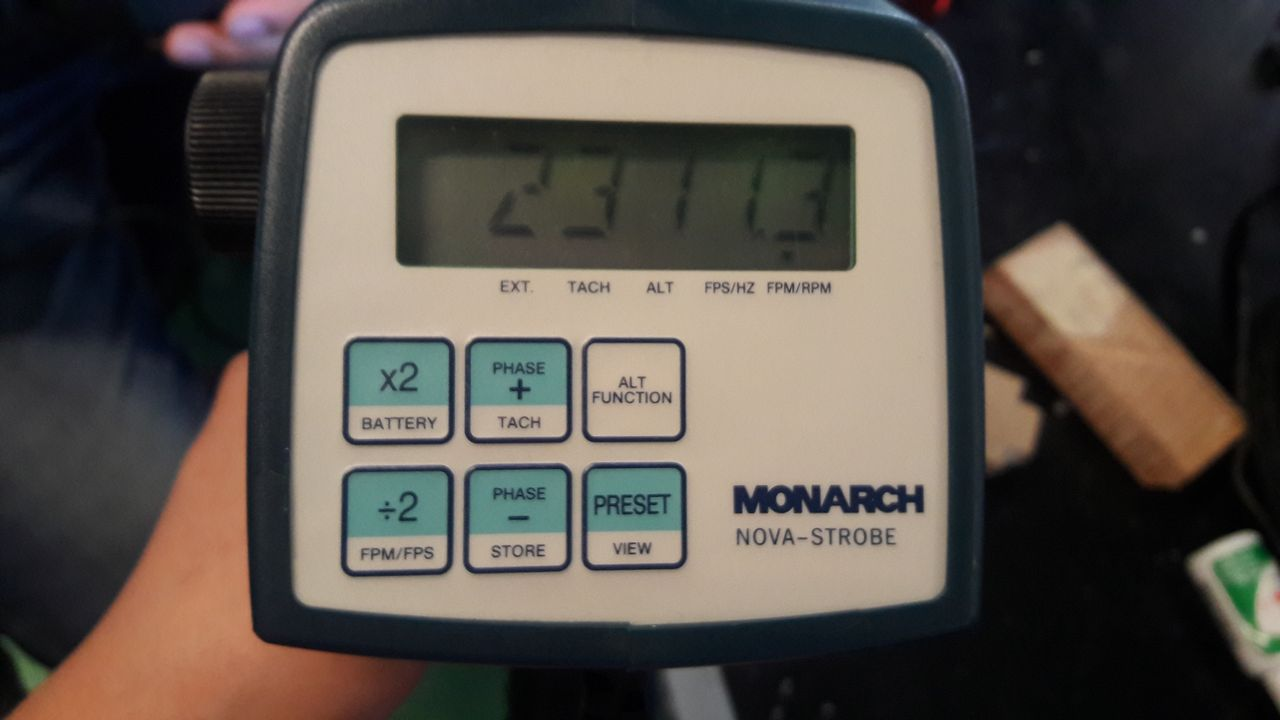
\includegraphics [scale=0.2]
 {./img/2311.jpg}
  \caption{Operaci\'on a 100\% de velocidad.}
 \end{figure}

  \begin{figure}[!htbp]
 \centering
 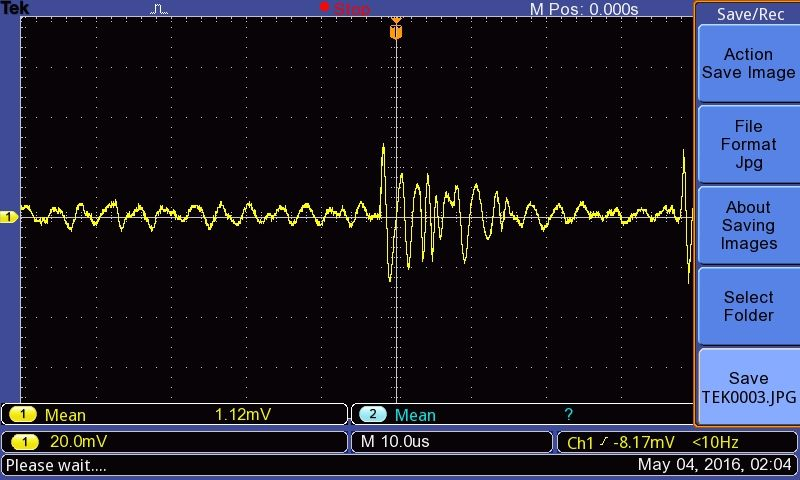
\includegraphics [scale=0.25]
 {./img/tek0003.jpg}
  \caption{Se\~nal a 100\% de velocidad.}
 \end{figure}

% \pagebreak